%%%%%%%%%%%%%%%%%%%%%%%%%%%%%%%%%%%%%%%%%%%%%%%
% Template baseado no exemplo da classe utftex
% Prof. César M. V. Benítez, Daniel Rossato
% DAELN, UTFPR-Curitiba (2020)
%%%%%%%%%%%%%%%%%%%%%%%%%%%%%%%%%%%%%%%%%%%%%%%


\documentclass[openright]{normas-utf-tex} %openright = o capitulo comeca sempre em paginas impares
%\documentclass[oneside]{normas-utf-tex} %oneside = para numero de paginas menor que 100 (apenas frente da folha) 

% force A4 paper format
\special{papersize=210mm,297mm}

\usepackage[alf,abnt-emphasize=bf,bibjustif,recuo=0cm, abnt-etal-cite=2, abnt-etal-list=99]{abntcite} %configuracao correta das referencias bibliograficas.

\usepackage[portuguese, ruled, linesnumbered]{algorithm2e}%pacotedealgoritmoemportugues

\usepackage[table]{xcolor}
\usepackage[brazil]{babel} % pacote portugues brasileiro
\usepackage[utf8]{inputenc} % pacote para acentuacao direta
\usepackage{amsmath,amsfonts,amssymb} % pacote matematico
\usepackage{graphicx} % pacote grafico
\usepackage{times} % fonte times
\usepackage[final]{pdfpages} % adicao da ata
\usepackage[version=3]{mhchem}%adição de pacote para quimica
% \usepackage{longtable}% redimensionar automaticamente tabelas
\usepackage{subfig}
\usepackage{relsize}
\usepackage[paper=portrait,pagesize]{typearea}
\usepackage{pdflscape}
\usepackage{url}

% minted
\usepackage{minted}

% adicionando bordas ao código em 'minted'
\usepackage{tcolorbox}
\usepackage{etoolbox}
\BeforeBeginEnvironment{minted}{\begin{tcolorbox}}%
\AfterEndEnvironment{minted}{\end{tcolorbox}}%


%\usepackage{hyperref}% link das res
\newcommand\tab[1][1cm]{\hspace*{#1}}

%Podem utilizar GEOMETRY{...} para realizar pequenos ajustes das margens. Onde, left=esquerda, right=direita, top=superior, bottom=inferior. P.ex.:
%\geometry{left=3.0cm,right=1.5cm,top=4cm,bottom=1cm} 
\usepackage{amsthm}
\newtheorem{mydef}{Definicão}

%\usepackage{balance} 



% ---------- Preambulo ----------
\instituicao{ UNIVERSIDADE TECNOLÓGICA FEDERAL DO PARANÁ (UTFPR)} % nome da instituicao
\programa{Projeto REA} % nome do programa
\area{Engenharia Mecânica} 
\documento{PROGRAMA DE APOIO AO DESENVOLVIMENTO DE RECURSOS EDUCACIONAIS ABERTOS NA GRADUAÇÃO DA UTFPR (ÁREAS TRANSVERSAIS)}
\nivel{Graduação em Engenharia Mecânica} 
\titulacao{Graduação em Engenharia Mecânica}

\titulo{RECURSOS DE INTERACAO EDUCACIONAL DIGITAL APLICADOS A FISICA, QUIMICA, A MATEMATICA E AS ENGENHARIAS USANDO O SCILAB E O PYTHON} % titulo do trabalho em portugues

% \title{\MakeUppercase{Título em Inglês}} % titulo do trabalho em ingles

\autor{Joe Michael Hideyuki Furuya Takahassi \protect} % autor do trabalho
%\cita{aluno1} % sobrenome (maiusculas), nome do autor do trabalho


\palavraschave{palavra chave}  % palavras-chave do trabalho
\keywords{keywords} % palavras-chave do trabalho em ingles

\comentario{Apostila elaborada para o projeto de Recursos Educacionais Abertos descritos no edital 26/2021 e ofertada pela UTFPR, apresentado aos avaliadores da banca como requisito para a conclusão do projeto.} 

\orientador{Prof. Dr. Antônio Carlos Amaro de Faria Júnior \protect} % nome do orientador do trabalho

\local{Curitiba} % cidade
\data{\the\year} % ano automatico

% desativa hifenizacao mantendo o texto justificado.
% thanks to Emilio C. G. Wille
\tolerance=1
\emergencystretch=\maxdimen
\hyphenpenalty=10000
\hbadness=10000
\sloppy

%---------- Inicio do Documento ----------
\begin{document}

\capa % geracao automatica da capa
\folhaderosto % geracao automatica da folha de rosto


% % dedicatoria (opcional)
% \begin{dedicatoria}
% Texto da dedicat\'oria. 
%\end{dedicatoria}

% % agradecimentos (opcional)
%\begin{agradecimentos}
% Texto dos agradecimentos.
%\end{agradecimentos}

% % epigrafe (opcional)
% \begin{epigrafe}
% Texto da ep\'igrafe.
% \end{epigrafe}

%resumo
%\begin{resumo}

% \end{resumo}

%abstract
% \begin{abstract}

% \end{abstract}

% listas (opcionais, mas recomenda-se a partir de 5 elementos)
\listadefiguras % geracao automatica da lista de figuras
\listadetabelas % geracao automatica da lista de tabelas
% \listadequadros % adivinhe :)
% \listadesiglas % geracao automatica da lista de siglas
% \listadesimbolos % geracao automatica da lista de simbolos

% sumario
\sumario % geracao automatica do sumario


%---------- Inicio do Texto ----------
% recomenda-se a escrita de cada capitulo em um arquivo texto separado (exemplo: intro.tex, fund.tex, exper.tex, concl.tex, etc.) e a posterior inclusao dos mesmos no mestre do documento utilizando o comando \input{}, da seguinte forma:
%\input{intro.tex}
%\input{fund.tex}
%\input{exper.tex}
%\input{concl.tex}

% Colocar aqui o numero da página inicial!!! (Obs.: conta a partir da folha de rosto)
\setcounter{page}{12}

\chapter{Introdução}

\section{Motivação} %qual o problema?
Esse material foi elaborado para o projeto "Recursos de Interação Educacional Digital Aplicados à Física, Química, à Matemática e às Engenharias usando o Scilab e o Python", ofertado pela UTFPR e pertencente ao Edital 26/2021. Para cada exemplo, foi exibido os respectivos códigos fontes assim como foi escrito uma explicação dos principais conceitos relacionados àquele tema. 

\section{Objetivos}
O objetivo do projeto é auxiliar o estudante no aprendizado de conceitos importantes tanto no campo da Física, Química, Matemática e Engenharias, através da elaboração de exemplos práticos no ambiente Jupyter Lab. Para isso, foi consultado referências bibliográficas para a elaboração da fundamentação teórica assim como foi utilizado algumas bibliotecas específicas do Python pertinentes para cada exemplo em questão.



%\subsection{Objetivo geral} 




%\subsection{Objetivos específicos} 
%\label{sec:objespecif}

   %Introducao
\chapter{Exemplos}

Nesta seção serão apresentados os exemplos práticos escolhidos para o projeto. 

\section{Exemplo de análise de tecnologia - Comunicação sem Fio}
\label{sec:exemplo}
Como mostrado na Seção \ref{sec:objespecif}, o projeto proposto necessita de um módulo de comunicação sem fio para interagir com o aplicativo no celular do usuário. Foram analisadas as tecnologias Wi-Fi e Bluetooth, visto que estas estão presentes em praticamente todos os \textit{smartphones} modernos.

\subsection{Wi-Fi}
\label{sec:wifi}

A tecnologia Wi-Fi é tecnologia de rede sem fio criada em 1998 pela Wi-Fi Alliance, baseada no padrão IEEE 802.11. Ela é hoje a tecnologia mais comum para conexão sem fio de dispositivos à internet em dispositivos pessoais \cite{WiFi2020}. Um dos módulos mais comuns para aplicações de \sigla{IoT}{Internet of Things} (Internet das Coisas) é o ESP8266 \cite{datasheet8266}, que tem baixo custo e fácil disponibilidade de compra. Este módulo é mostrado na Figura \ref{fig:esp8266}.

\begin{figure}[!htb]
	\centering
	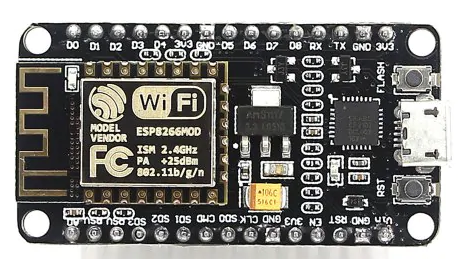
\includegraphics[width=0.4\textwidth]{./esp8266.png} 
	\caption{Foto do módulo Wi-Fi ESP8266.}
	\label{fig:esp8266}
\end{figure}

\subsection{Bluetooth}
\label{sec:bt}
A tecnologia Bluetooth foi criada em 1989, com o objetivo de substituir o protocolo RS-232 na comunicação de curta distância entre objetos fixos (citar referência). O módulo mais comum para IoT é o HC-05, mostrado na Figura \ref{fig:hc05}.

\begin{figure}[!htb]
	\centering
	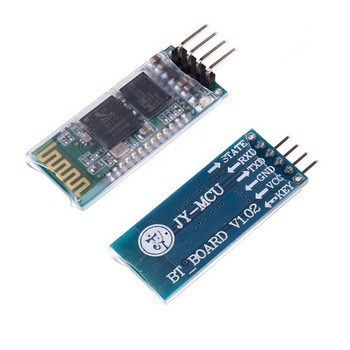
\includegraphics[width=0.4\textwidth]{./hc05.jpg} 
	\caption{Foto do módulo Bluetooth HC-05.}
	\label{fig:hc05}
\end{figure}

\subsection{Comparativo entre tecnologias de comunicação sem fio}
Na Tabela \ref{tab:semfio} são comparadas as principais características dos módulos ESP8266 e HC-05. Esta tabela foi criada com o auxílio do site \url{www.tablesgenerator.com}.

\begin{table}[!htb]
\centering
\begin{tabular}{l|l|l}
    ~       & ESP8266   & HC-05      \\
    \hline
    Alcance & 50m       & 10m        \\
    \hline
    Consumo & 170mA     & 40mA       \\
    \hline
    Preço   & R\$ 22,90 & R\$ 25,90  \\
    \hline
\end{tabular}
\caption{Comparativo entre módulos ESP8266 e HC-05}
\label{tab:semfio}
\end{table}

O módulo ESP8266 tem maior alcance e menor custo que o HC-05, como pode ser visto na Tabela \ref{tab:semfio}. Porém, como o projeto proposto será alimentado por bateria, é essencial diminuir o consumo de corrente do sistema. Por isso, foi escolhido o módulo HC-05. Além disso, o desenvolvimento de aplicações com comunicação Bluetooth já é dominado pela equipe, reduzindo a dificuldade da implementação.



   %Fundamentacao teorica
\chapter{Metodologia}

\section{Visão geral}


* Obs.: nao esqueça de apresentar o diagrama de blocos do sistema. 


\section{Projeto mecânico}


\section{Projeto de \textit{hardware}}


* Obs.: nao esqueça de apresentar o diagrama de blocos do hardware. 


\section{Projeto de \textit{software}}



* Obs.: nao esqueça de apresentar os diagramas de estados (statecharts) do 
software.


\section{Integração}









   %Metodologia
\chapter{Experimentos e resultados}

% testes, integração, etc.   %Experimentos e resultados
\section{Distribuição Gaussiana}

\subsection{O que é a Distribuição Gaussiana?}
A \textbf{distribuição Gaussiana} ou \textbf{distribuição normal} é uma das distribuições mais importantes em razão da sua enorme presença nos mais variados campos do conhecimento. Se trata de uma curva de distribuição simétrica em torno do seu ponto médio. Ela possui a peculiaridade de ter a média, mediana e moda dos dados com o mesmo valor.

\subsection{Variável aleatória]}
\textbf{Variável aleatória} é um valor retirado de uma distribuição estatística e que não possui um valor fixo. O seu valor depende de fatores aleatórios. Ex: o resultado do lançamento de um dado pode dar qualquer número entre 1 e 6.

Uma variável aleatória que pode assumir apenas um número finito ou uma sequência infinita enumerável de valores é considerada \textbf{discreta}. Aquele que pode assumir qualquer valor no intervalo dos números reais é considerado \textbf{contínuo}. 

Uma \textbf{variável aleatória contínua} é uma variável aleatória que pode tomar qualquer valor numérico em um determinado intervalo ou coleção de intervalos (geralmente do conjunto dos números reais). Ex: uma variável aleatória que mede o tempo que leva para algo ser feito é contínua, pois ela pode assumir infinitos valores.

Como existe um número infinito de valores em qualquer intervalo, não faz sentido falar sobre a probabilidade da variável aleatória assumir um valor específico. Em vez disso, é considerada a probabilidade de uma variável aleatória contínua estar dentro de um determinado intervalo. É a chamada \textbf{Função Densidade de Probabilidade}.

\subsection{Função Densidade de Probabilidade}

É a função $f(x)$  de uma variável aleatória contínua cuja integral em um intervalo dá a probabilidade de que o valor da variável esteja dentro desse mesmo intervalo. Ou seja, \textbf{densidade de probabilidade} não é probabilidade. Somente quando a função for integrada entre dois limites é que ela produzirá uma probabilidade, sendo equivalente à área sob a curva da função densidade de probabilidade entre esses dois limites:

\[\large \int_{a}^{b} f(x)dx = P(a\leq x\leq b)\]

As funções densidade de probabilidade devem sempre obedecer à esses 2 requisitos:
\begin{itemize}
\item $f(x)$ deve ser não negativo para cada valor da variável aleatória: $f(x) > 0$
\item A área total sob a curva de probabilidade vale sempre 1: $\int_{-\infty }^{\infty} f(x)dx = 1$
\end{itemize}

A forma da função de densidade de probabilidade em todo o seu domínio é chamada de \textbf{distribuição de probabilidade}. A distribuição de probabilidade mais importante é a chamada \textbf{distribuição normal}, também chamado de \textbf{curva em forma de sino} devido à sua forma característica.

\subsection{Distribuição Normal ou Gassiana}

A distribuição normal é a distribuição de probabilidade mais importante no estudo da estatística devido à sua presença em muitos fenômenos naturais, por exemplo: a altura das pessoas, pressão arterial, erro de medição e pontuações de QI seguem a distribuição normal.

Como já foi dito, a probabilidade de uma observação assumir um valor entre dois pontos quaisquer é igual à área sob a curva da densidade de probabilidade compreendida entre esses dois pontos. No caso de uma curva de distribuição normal teórica, a regra é: 

\begin{itemize} 

\item $68,26\%$ da população ou amostra está dentro de uma região que varia de $\mu \pm \sigma$ 
\item $95,44\%$ da população ou amostra está dentro de uma região que varia de $\mu \pm 2\sigma$
\item $99,72\%$ da população ou amostra está dentro de uma região que varia de $\mu \pm 3\sigma$
\item $99,99\%$ da população ou amostra está dentro de uma região que varia de $\mu \pm 4\sigma$ 

\end{itemize}

\begin{figure}[H]
	\centering
	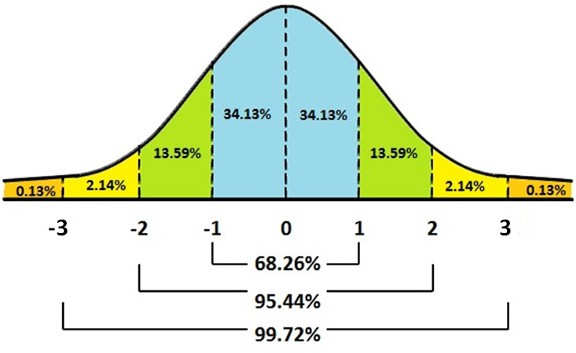
\includegraphics[width=1\textwidth]{./Imagens/Distribuição Normal/GA1.png} 
	\caption{Distribuição normal}
	\label{fig:GA1}
\end{figure}

\subsection{Densidade para a distribuição normal}
Uma variável aleatória contínua X tem distribuição normal se sua função densidade de probabilidade for dada por:

\[ \large p(x) = \frac{1}{\sigma \sqrt{2 \pi  }}e^{-\frac{1}{2} (\frac{x-\mu}{\sigma})^2} \]

Onde $\sigma$ é o \textbf{desvio padrão} da distribuição e $\mu$ é a \textbf{média}.

\subsection{Desvio padrão}

Comumente representado pelo símbolo $\sigma$, é uma medida de dispersão em torno da média populacional ou amostral de uma variável aleatória. Quanto maior o seu valor maior a ampla de valores na qual os dados estão espalhados. Um baixo desvio padrão indica que os pontos dos dados tendem a estar próximos da média.

\subsection{Fórmula para o desvio padrão}

O desvio padrão populacional ou amostral é a raiz quadrada da variância populacional ou amostral correspondente. 

\begin{itemize}

\item Quando o conjunto de dados é a população:

\[ \large \sigma = \sqrt{\frac{1}{N}\sum_{i=1}^{N}(x_{i}-\mu )^2} \]

\item Quando o conjunto de dados é uma amostra:

\[ \large \sigma = \sqrt{\frac{1}{N-1}\sum_{i=1}^{N}(x_{i}-\mu )^2} \]

\end{itemize}

\subsection{Distribuição Normal no Python}

Vamos traçar a curva de uma \textbf{distribuição normal padronizada}, que é uma curva normal de média $\mu = 0$ e desvio padrão $\sigma = 1$.

\begin{minted}{python}
	
from scipy.stats import norm
import matplotlib.pyplot as plt
import numpy as np 

fig, ax = plt.subplots(figsize = (8,5))

# definindo o domínio
dom = np.linspace(-2,2,1000)

plt.plot(dom, norm.pdf(dom, loc = 0 , scale = 1))
plt.title("Distribuição Normal Padronizada")
plt.xlabel("Valor")
plt.ylabel("Densidade")
ax.grid(True)
plt.show()

\end{minted}

\begin{figure}[H]
	\centering
	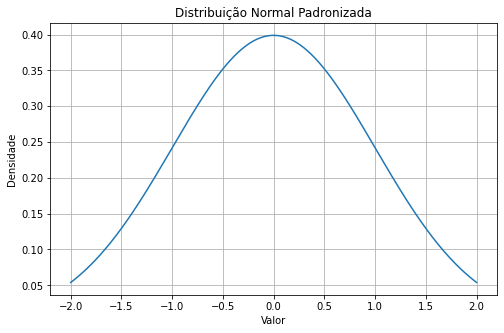
\includegraphics[width=1\textwidth]{./Imagens/Distribuição Normal/GA2.png} 
	\caption{Curva normal}
	\label{fig:GA2}
\end{figure}

Podemos alterar a forma da curva em sino alterando a média e o seu desvio padrão. Alterar a média deslocará a curva em direção a esse valor, isso significa que podemos alterar a posição da curva alterando o valor médio sem afetar a forma da curva.

\begin{minted}{python}
	
fig, ax = plt.subplots(figsize = (8,5))

x = np.linspace(-10,15,100)

medias = [0.0, 2.0, 5.0, 10.0]

for medias in medias:
ax.plot(x, norm.pdf(x,loc=medias), label=f"Médias: {medias}")

ax.set_xlabel('x')
ax.set_ylabel('pdf(x)')
ax.set_title('Distribuição Normal')
ax.legend(loc='best', frameon=True)
ax.set_ylim(0,0.45)
ax.grid(True)
	
\end{minted}

\begin{figure}[H]
	\centering
	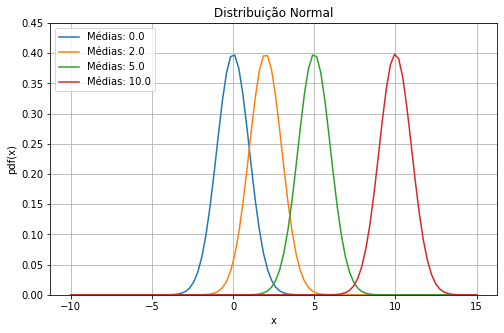
\includegraphics[width=1\textwidth]{./Imagens/Distribuição Normal/GA3.png} 
	\caption{Alterando a média}
	\label{fig:GA3}
\end{figure}

A forma da curva pode ser controlada pelo valor do desvio padrão. Um desvio padrão menor resultará em uma curva estreitamente limitada, enquanto um valor alto resultará em uma curva mais espalhada. 

\begin{minted}{python}
	
fig, ax = plt.subplots(figsize = (8,5))

x = np.linspace(-10,10,100)

stdvs = [1.0, 2.0, 3.0, 4.0]

for s in stdvs:
ax.plot(x, norm.pdf(x, scale=s), label=f'desvio padrão = {s}')

ax.set_xlabel('x')
ax.set_ylabel('pdf(x)')
ax.set_title('Distribuição Normal')
ax.legend(loc='best', frameon=True)
ax.set_ylim(0,0.45)
ax.grid(True)
	
\end{minted}

\begin{figure}[H]
	\centering
	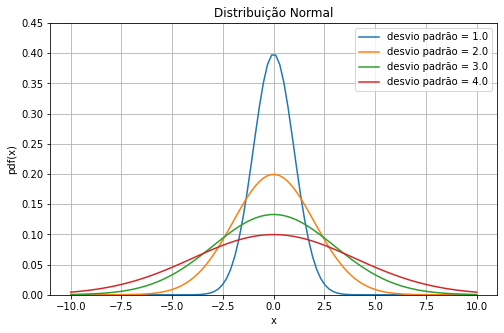
\includegraphics[width=1\textwidth]{./Imagens/Distribuição Normal/GA4.png} 
	\caption{Alterando o desvio padrão}
	\label{fig:GA4}
\end{figure}

\subsection{Função distribuição acumulada}

É a função $F(x)$ que indica a probabilidade de um determinado valor de uma variável aleatória X ser menor ou igual à x. Em termos matemáticos:

\[\large F(x) = P(X \leq x) = \int_{-\infty }^{x}f(x_{i})dx\]

\subsubsection{Calculando a probabilidade de ocorrência de dados específicos}

Vamos utilizar o conceito de função distribuição acumulada (CDF) e calcular a probabilidade de um valor estar abaixo de -1 ao escolhermos um valor aleatório da distribuição. Essa probabilidade será a área da região apresentada abaixo e terá um valor de aproximadamente $15,87\%$.

\begin{figure}[H]
	\centering
	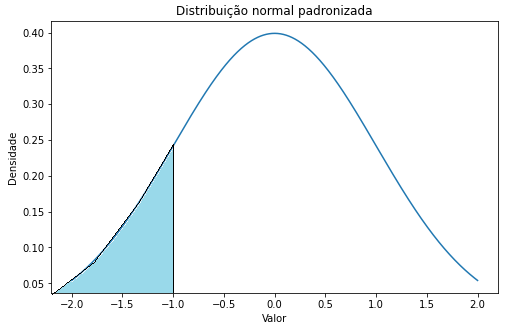
\includegraphics[width=1\textwidth]{./Imagens/Distribuição Normal/GA5.png} 
	\caption{Abaixo de -1}
	\label{fig:GA5}
\end{figure}

\begin{minted}{python}
prob = norm(loc = 0 , scale = 1).cdf(-1)
print(f"Probabilidade: {prob*100:.2f}%")
# Probabilidade: 15.87%
\end{minted}

Para calcular a probabilidade do valor estar entre uma região específica (entre 2 e 1 por exemplo):

\begin{figure}[H]
	\centering
	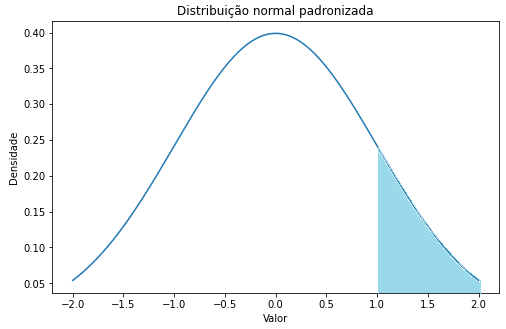
\includegraphics[width=1\textwidth]{./Imagens/Distribuição Normal/GA6.png} 
	\caption{Entre 1 e 2}
	\label{fig:GA6}
\end{figure}

\begin{minted}{python}
cdf_limite_superior = norm(loc = 0 , scale = 1).cdf(2)
cdf_limite_inferior = norm(loc = 0 , scale = 1).cdf(1)

prob = cdf_limite_superior - cdf_limite_inferior
print(f"Probabilidade: {prob*100:.2f}%")
# Probabilidade: 13.59%
\end{minted}

Para calcular a probabilidade do valor ser maior que x (0.5 por exemplo): 

\begin{figure}[H]
	\centering
	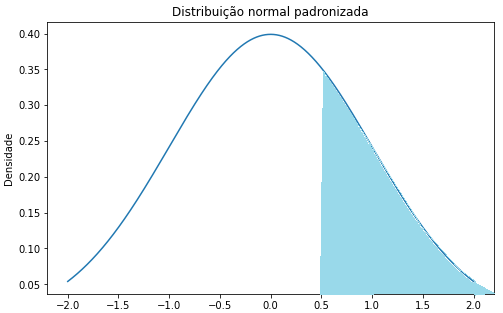
\includegraphics[width=1\textwidth]{./Imagens/Distribuição Normal/GA7.png} 
	\caption{Maior que 0.5}
	\label{fig:GA7}
\end{figure}

\begin{minted}{python}
prob = 1 - norm(loc = 0 , scale = 1).cdf(0.5)
print(f"Probabilidade: {prob*100:.2f}%")
# Probabilidade: 30.85%
\end{minted}

\subsection{Aplicações da Distribuição Normal}
\begin{itemize}
\item O matemático francês Abraham de Moivre, em seu Doctrine of Chances (1718), primeiro observou que as probabilidades associadas a variáveis aleatórias geradas discretamente (como as obtidas jogando uma moeda ou jogando um dado) podem ser aproximadas pela área sob o gráfico de uma função exponencial. Este resultado foi estendido e generalizado pelo cientista francês Pierre-Simon Laplace.
\item Em 1860, Maxwell supôes que a velocidade das colisões das partículas obedecem a distribuição normal.
\item Pode ser utilizado na análise da resistência dos materiais, onde os dados coletados podem ser generalizados para uma distribuição normal de forma a facilitar as simulações computacionais e torná-los mais práticos. 
\item Em projetos de engenharia no campo da ergonomia.
\end{itemize}   %Cronograma e custos do projeto
\section{Integral de Riemann}

\subsection{Conceito de Integral}

Em cálculo, o conceito de integral se refere à soma infinitesimal de regiões para se obter o valor total de uma região contínua. Ela pode ser considerada uma área ou a generalização de uma área e, juntamente com a derivada, constitui os conceitos fundamentais do Cálculo.

O exemplo mais simples de integral é a \textbf{Integral de Riemann}. Considerando uma função contínua $f(x)$ num intervalo $[a,b]$ tal que $f(x) \geq 0$  para todo $x \; \epsilon \; [a,b]$, a sua curva plotada no sistema cartesiano fica:

\begin{figure}[H]
	\centering
	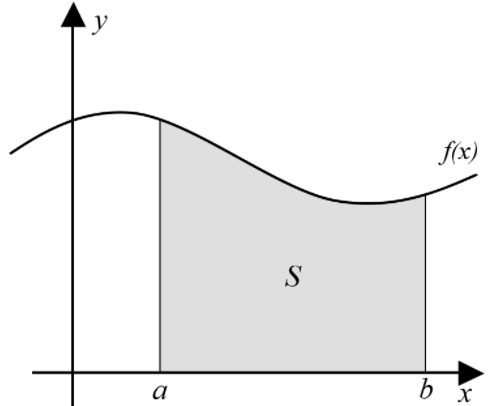
\includegraphics[width=0.8\textwidth]{./Imagens/Integral de Riemann/RI1.png} 
	\caption{Área sob a curva}
	\label{fig:RI1}
\end{figure}

\subsection{Integral de Riemann}

O valor total da área sob a curva da função $f(x)$ pode ser obtido dividindo essa área em diversos retângulos menores com extremidades nos pontos $[x_{0}, x_{1}, x_{2}, x_{3}, ..., x_{n}]$. A fórmula para a Integral de Rieman basicamente diz que a área da região compreendida entre o eixo horizontal e o gráfico da função $f(x)$, para x percorrendo o intervalo $[a,b]$, é igual ao limite da soma das áreas dos $n$ retângulos, quando o número desses retângulos tende a infinito.

\begin{figure}[H]
	\centering
	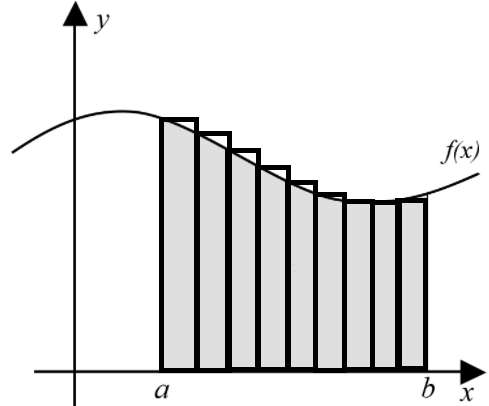
\includegraphics[width=0.8\textwidth]{./Imagens/Integral de Riemann/RI2.png} 
	\caption{Divisão da área}
	\label{fig:RI2}
\end{figure}

\subsubsection{Fórmula}

A Integral de Riemann da função $f(x)$ em relação a $x$ de $a$ para $b$ é: 

\begin{equation}
\large \int_{a}^{b}f(x) \; dx = \lim_{n \rightarrow \infty}\sum_{i=1}^{n} \frac{b-a}{n}f(x_{i-1})
\tag{5.1}
\end{equation}

A integral corresponde à "área com sinal", isto é, a área acima do eixo $x$ é positiva e a área abaixo do eixo $x$ é negativa.

Quando ela possui 2 limites, a integral é do tipo \textbf{definida}. Integral sem limite é denominada \textbf{indefinida}.

\subsection{Função primitiva/integral indefinida/antiderivada}

A \textbf{função primitiva/integral indefinida/antiderivada} de uma função $f$ é uma função diferenciável $F$ cuja derivada é igual à função original $f$. Isso pode ser representado simbolicamente por $F' = f$.

O processo de calcular funções primitivas (ou integrais indefinidas) de funções é oposto ao da diferenciação de funções, cujo objetivo é obter a derivada. Funções primitivas geralmente são representados por letras maiúsculas e estão relacionadas às integrais definidas pelo \textbf{Teorema Fundamental do Cálculo}.

Exemplo: 

A função $F(x) = \frac{x^3}{3}$ é a função primitiva de $f(x) = x^2$ uma vez que a derivada de $F(x) = \frac{x^3}{3}$ é $x^2$. Uma vez que a derivada de uma constante é zero, $x^2$ possuirá infinitas funções primitivas da forma $F(x) = \frac{x^3}{3} + C$ onde $C$ é denominada constante de integração.

\subsection{Teorema Fundamental do Cálculo}

O \textbf{Teorema Fundamental do Cálculo} diz que se $f(x)$ é uma função contínua em $[a,b]$, a sua integral definida nesse intervalo é a diferença entre as suas funções primitivas $F(x)$ nas extremidades desse intervalo:

\begin{equation}
\large \int_{b}^{a}f(x)\:dx = F(b) - F(a) = F(x)|^{b}_{a}
\tag{5.2}
\end{equation}

\subsection{Integral de Riemann utilizando scipy do Python}
Vamos utilizar a função \textbf{quad} da biblioteca Scipy para realizar a integração da função abaixo:

\begin{equation}
\large \int_{0}^{4}x^2dx
\tag{5.3}
\end{equation}

Para isso, vamos utilizar a função \textbf{lambda} do Python, que permite a criação de funções com número qualquer de argumentos:

\begin{minted}{python}
	x2 = lambda x: x**2
	print(x2)
	print(type(x2))
\end{minted}

Após isso, usamos a a função \textbf{integrate} da biblioteca \textbf{scipy} para realizar a integração.

O valor retornado pela função é uma tupla, onde o primeiro elemento é o valor estimado da integral e o segundo elemento é o limite superior de erro.

\begin{minted}{python}
	from scipy import integrate
	integrate.quad(x2, 0, 4)
\end{minted}

\begin{equation}
\large \int_{0}^{4}x^2dx \cong 21.333
\tag{5.4}
\end{equation}

\subsection{Exemplo por aproximação superior}

Vamos resolver a mesma integral de Riemann por aproximação superior. Para isso, vamos dividir a área S em diversos retângulos de base $[x_{i-1},x_{i}]$ e altura $f(x_{i})$

\begin{minted}{python}
import matplotlib.pyplot as plt
import numpy as np

fig, ax = plt.subplots(figsize =(8,6))

a = 0
b = 4
n = 5
x = np.linspace(a,b,n+1)

f = lambda x: x**2
vetor = []

for i in x:
	vetor.append(f(i))
	plt.vlines(i,0,f(i))

y = x**2
plt.plot(x,y)
plt.bar(x, vetor, align='edge', width=-(b-a)/n, 
color='pink')
plt.show()
\end{minted}

\begin{figure}[H]
	\centering
	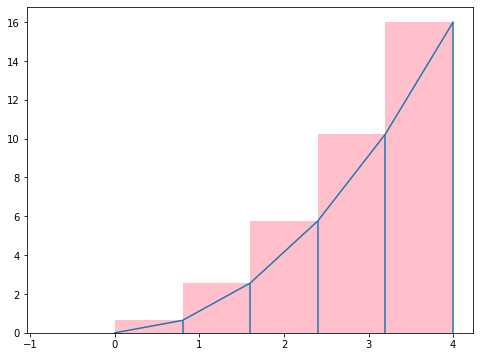
\includegraphics[width=0.8\textwidth]{./Imagens/Integral de Riemann/RI3.png} 
	\caption{Aproximação superior}
	\label{fig:RI3}
\end{figure}

A área da região S será tanto mais próxima do valor real $21.333$ quanto mais retângulos utilizarmos para dividir a área:

\begin{minted}{python}
import numpy as np

def area(a,b,n):
y = np.linspace(a,b,n+1)
w = (b - a)/n
f = lambda x: x**2
S = 0

for i in y[1:]:
	S = S + f(i)*w 
	
	print(f"Área: {S:.3f} (para {n} retângulos)")

area(0,4,5)
# Área: 28.160 (para 5 retângulos)
area(0,4,100)
# Área: 21.654 (para 100 retângulos)
area(0,4,500)
# Área: 21.397 (para 500 retângulos)
area(0,4,1000)
# Área: 21.365 (para 1000 retângulos)
area(0,4,5000)
# Área: 21.340 (para 5000 retângulos)
area(0,4,10000)
# Área: 21.337 (para 10000 retângulos)

\end{minted}

\subsection{Exemplo por aproximação inferior}

Vamos resolver a mesma integral de Riemann por aproximação inferior. Para isso, vamos dividir a área S em diversos retângulos de base $[x_{i-1},x_{i}]$ e altura $f(x_{i-1})$

\begin{minted}{python}
import matplotlib.pyplot as plt

fig, ax = plt.subplots(figsize =(8,6))

a = 0
b = 4
n = 5
x = np.linspace(a,b,n+1)

f = lambda x: x**2
vetor = []
for i in x:
	vetor.append(f(i))
	plt.vlines(i,0,f(i))

y = x**2
plt.plot(x,y)
plt.bar(x[:-1], vetor[:-1], align='edge', 
width=(b-a)/n, color='pink')
plt.show()
\end{minted}

\begin{figure}[H]
	\centering
	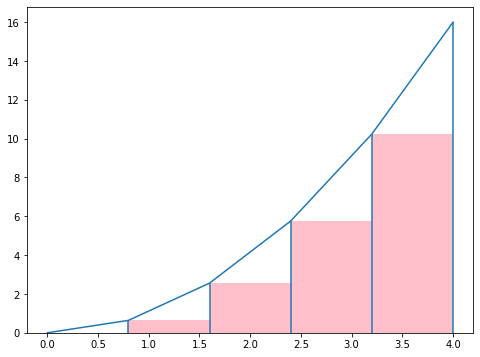
\includegraphics[width=0.8\textwidth]{./Imagens/Integral de Riemann/RI4.png} 
	\caption{Aproximação inferior}
	\label{fig:RI4}
\end{figure}

A área da região S será tanto mais próxima do valor real $21.333$ quanto mais retângulos utilizarmos para dividir a área:

\begin{minted}{python}
import numpy as np

def area(a,b,n):
y = np.linspace(a,b,n+1)
w = (b - a)/n
f = lambda x: x**2
S = 0

for i in y[:-1]:
	S = S + f(i)*w 

	print(f"Área: {S:.3f} (para {n} retângulos)")

area(0,4,5)
# Área: 15.360 (para 5 retângulos)
area(0,4,100)
# Área: 21.014 (para 100 retângulos)
area(0,4,500)
# Área: 21.269 (para 500 retângulos)
area(0,4,1000)
# Área: 21.301 (para 1000 retângulos)
area(0,4,5000)
# Área: 21.327 (para 5000 retângulos)
area(0,4,10000)
# Área: 21.330 (para 10000 retângulos)
\end{minted}

\subsection{Aplicações da Integral de Riemann}

\begin{itemize}
\item Pode ser utilizado na Matemática para: determinar a área de polígonos regulares ou irregulares; calcular a Transformada de Fourier; determinar o comprimento de uma curva; determinar o volume de um sólido.
\item Na física, é utilizado para: determinar a massa de um objeto caso a sua densidade seja conhecida; calcular o trabalho realizado partindo da força; calcular a velocidade e o instante dado a aceleração e as condições iniciais; calcular as equações de Maxwell.
\item Na engenharia é utilizado para determinar a força cortante e momento fletor; centroide de uma área; momento de inércia de uma área;
\item Na estatística é utilizado na função densidade de probabilidade.
\item Na química, pode ser utilizado para determinar a força a partir da pressão provocada por um conjunto de moléculas no interior de um recipiente.
\end{itemize}
   %Conclusoes e trabalhos futuros






%---------- Referencias ----------
\clearpage % this is need for add +1 to pageref of bibstart used in 'ficha catalografica'.
\label{bibstart}
\bibliography{reflatex} % geracao automatica das referencias a partir do arquivo reflatex.bib
\label{bibend}

% %---------- Apendices (opcionais) ----------
% \apendice
% \chapter{Nome do Ap\^endice}

% Use o comando {\ttfamily \textbackslash apendice} e depois comandos {\ttfamily \textbackslash chapter\{\}}
% para gerar t\'itulos de ap\^en-dices.


% % ---------- Anexos (opcionais) ----------
% \anexo
% \chapter{Nome do Anexo}

% Use o comando {\ttfamily \textbackslash anexo} e depois comandos {\ttfamily \textbackslash chapter\{\}}
% para gerar t\'itulos de anexos.


% --------- Ordenacao Afabetica da Lista de siglas --------
%\textbf{* Observações:} a ordenacao alfabetica da lista de siglas ainda nao eh realizada de forma automatica, porem
% eh possivel se de realizar isto manualmente. Duas formas:
%
% ** Primeira forma)
%    A ordenacao eh feita com o auxilio do comando 'sort', disponivel em qualquer
% sistema Linux e UNIX, e tambem em sistemas Windows se instalado o coreutils (http://gnuwin32.sourceforge.net/packages/coreutils.htm)
% comandos para compilar e ordenar, supondo que seu arquivo se chame 'dissertacao.tex':
%
%      $ latex dissertacao
%      $ bibtex dissertacao && latex dissertacao
%      $ latex dissertacao
%      $ sort dissertacao.lsg > dissertacao.lsg.tmp
%      $ mv dissertacao.lsg.tmp dissertacao.lsg
%      $ latex dissertacao
%      $ dvipdf dissertacao.dvi
%
%
% ** Segunda forma)
%\textbf{Sugest\~ao:} crie outro arquivo .tex para siglas e utilize o comando \sigla{sigla}{descri\c{c}\~ao}.
%Para incluir este arquivo no final do arquivo, utilize o comando \input{arquivo.tex}.
%Assim, Todas as siglas serao geradas na ultima pagina. Entao, devera excluir a ultima pagina da versao final do arquivo
% PDF do seu documento.


%-------- Citacoes ---------
% - Utilize o comando \citeonline{...} para citacoes com o seguinte formato: Autor et al. (2011).
% Este tipo de formato eh utilizado no comeco do paragrafo. P.ex.: \citeonline{autor2011}

% - Utilize o comando \cite{...} para citacoeses no meio ou final do paragrafo. P.ex.: \cite{autor2011}



%-------- Titulos com nomes cientificos (titulo, capitulos e secoes) ----------
% Regra para escrita de nomes cientificos:
% Os nomes devem ser escritos em italico, 
%a primeira letra do primeiro nome deve ser em maiusculo e o restante em minusculo (inclusive a primeira letra do segundo nome).
% VEJA os exemplos abaixo.
% 
% 1) voce nao quer que a secao fique com uppercase (caixa alta) automaticamente:
%\section[nouppercase]{\MakeUppercase{Estudo dos efeitos da radiacao ultravioleta C e TFD em celulas de} {\textit{Saccharomyces boulardii}}
%
% 2) por padrao os cases (maiusculas/minuscula) sao ajustados automaticamente, voce nao precisa usar makeuppercase e afins.
% \section{Introducao} % a introducao sera posta no texto como INTRODUCAO, automaticamente, como a norma indica.

%\balance
\end{document}
